%****************************************************************%
% FILE: osservaizoni_satellite.tex                               %
%****************************************************************%
\documentclass[./main.tex]{subfiles}

\begin{document}

Le osservazioni da satellite richieste per l'applicazione sono relative all'osservazione della temperatura superficiale e della clorofilla presenti nel mar Mediterraneo in un'area geografica circoscritta. I dati sono disponibili in un catalogo THREEDS aggiornato.\par

\noindent \begin{minipage}{0.5\textwidth}
\vspace{1cm}
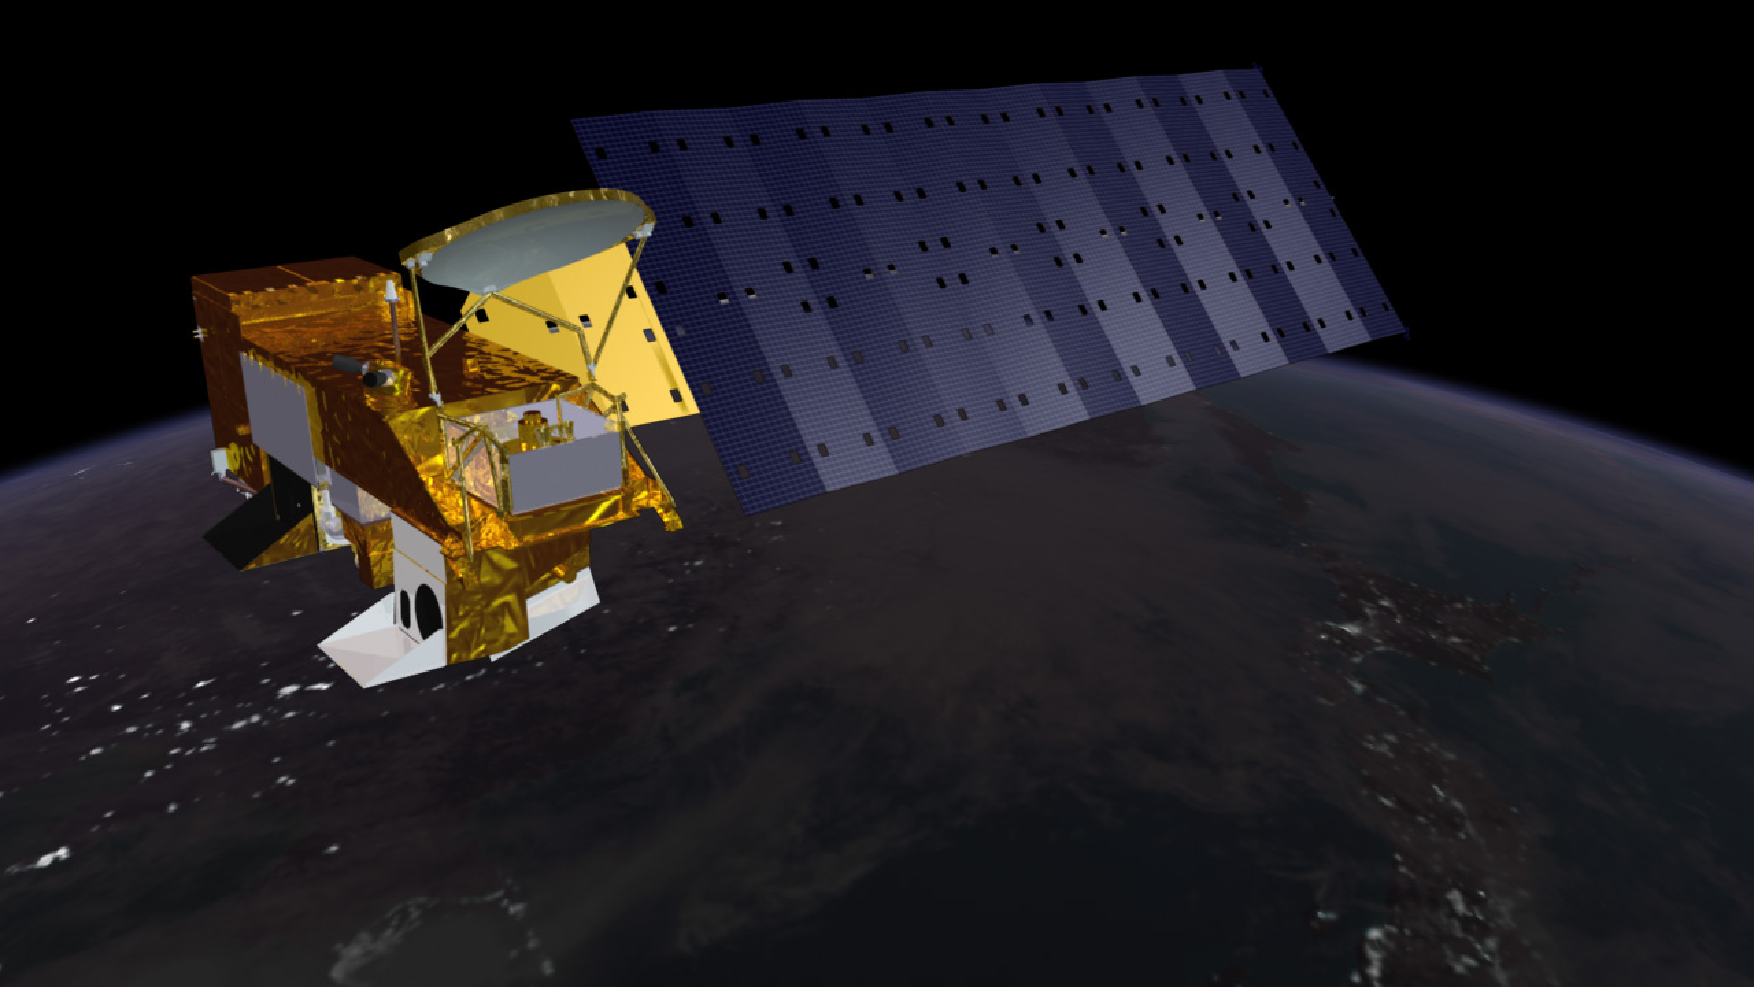
\includegraphics[width=\textwidth]{images/aqua_render_lrg.pdf}
\captionsetup{font=small, hypcap=false}
\captionof{figure}{Satellite Acqua NASA\footcite[Fonte: ][\url{https://upload.wikimedia.org/wikipedia/commons/f/fb/The_Aqua_Satellite.pdf}]{img-satellite-aqua}.}
\label{fig:aqua}
\end{minipage}
\hspace{0.05\textwidth}
\begin{minipage}{0.4\textwidth}
\begin{small}
Il satellite Aqua orbita a 705km\footcite[\url{{https://aqua.nasa.gov/content/about-aqua}}]{website-satellite-aqua} sopra la terra e trasporta una serie di sensori progettati per il monitoraggio dell'acqua e dell'atmosfera sul pianeta Terra.
\end{small}
\end{minipage}
\vspace{0.25cm}

%****************************************************************%
% clorofilla                                                     %
%****************************************************************%
\paragraph{Clorofilla-a (Chla).}
La clorofilla rappresenta il pigmento fotosintetico predominante nel fitoplancton\footnote{\textbf{fitoplàncton} s. m. [comp. di fito- e plancton]. – In ecologia, l’insieme degli organismi vegetali che costituiscono il plancton; si distinguono un f. d’acqua dolce e un f. marino, costituiti da cloroficee, diatomee, dinoflagellati, ecc; \cite{treccani-fitoplancton}.
}. La \textit{concentrazione di clorofilla-a} (\textbf{Chla}) è una variabile climatica che  indica l'abbondanza del fitoplancton e il colore dell'oceano. Queste osservazioni permettono di comprendere la variabilità del fitoplancton, stato di eutrofizzazione\footnote{\textbf{eutrofiżżazióne} s. f. [der. di eutrofico]. – In ecologia, il processo per cui una massa d’acqua (per es. un lago) diventa più eutrofica, sia per mutazione naturale sia per fertilizzazione artificiale, per es. da inquinamento; quest'ultima, detta e. colturale, è dovuta, fondamentalmente, ad accumulo di grosse quantità di sali fosforici provenienti da detersivi o da fertilizzanti, e di composti azotati presenti nei fertilizzanti stessi e nelle acque luride, ed è causa delle cosiddette fioriture di fitoplancton; \cite{treccani-eutrofizzazione}.
} e qualità dell'acqua. Dunque Chla risulta essere una delle variabili climatiche essenziali per caratterizzare il clima del pianeta\footcite{MERDER2024198}.

%\paragraph{Variabile osservata.} 
La Chla viene rilevata da satellite utilizzando appositi algoritmi empirici (non analizzati nel presente documento) indicati come \textit{algoritmi del colore dell'oceano}\footcite{dierssen2010perspectives} (\textbf{OC}). I dati vengono prelevati ed elaborati tramite l'unione delle informazioni provenienti da diversi sensori, col cosiddetto \textit{approccio multi-sensore}, per aumentare la probabilità di osservazioni valide di cielo sereno\footcite[129-132]{os-15-127-2019}. Le osservazioni si concentrano nell'area geo-spaziale rappresentante il mare italiano, delimitata da:
\begin{itemize}
    \item \textit{Longitudine}: da 7.0 a 20.0 Risoluzione=0.012 gradi est
    \item \textit{Latitudine}: da 35.0 a 46.0 Risoluzione=0.012 gradi nord 
\end{itemize}

%\paragraph{Misurazioni.} 
I dati sono disponibili in un catalogo THREDDS\footcite[\url{http://ritmare.artov.ismar.cnr.it/thredds/ritmare/SatelliteOS/OC/catalog.html?dataset=CHL_CASE12_A}]{thredds-chla} aggiornato contenente le variabili osservate in formato standard NetCDF-4\footcite[19-47]{HFR_QC_JERICO}. La concentrazione di clorofilla è misurata in  $milligram$ $m^{-3}$. È presente un visualizzatore web (\textit{GODIVA2}) che consente la visualizzazione grafica dei dati provenienti dal dataset\footcite{blower2009godiva2}. Un esempio è mostrato in \autoref{fig:godiva_chla}.

\begin{figure}[!ht]
\noindent\begin{minipage}{\textwidth}
\vspace{1cm}
\centering
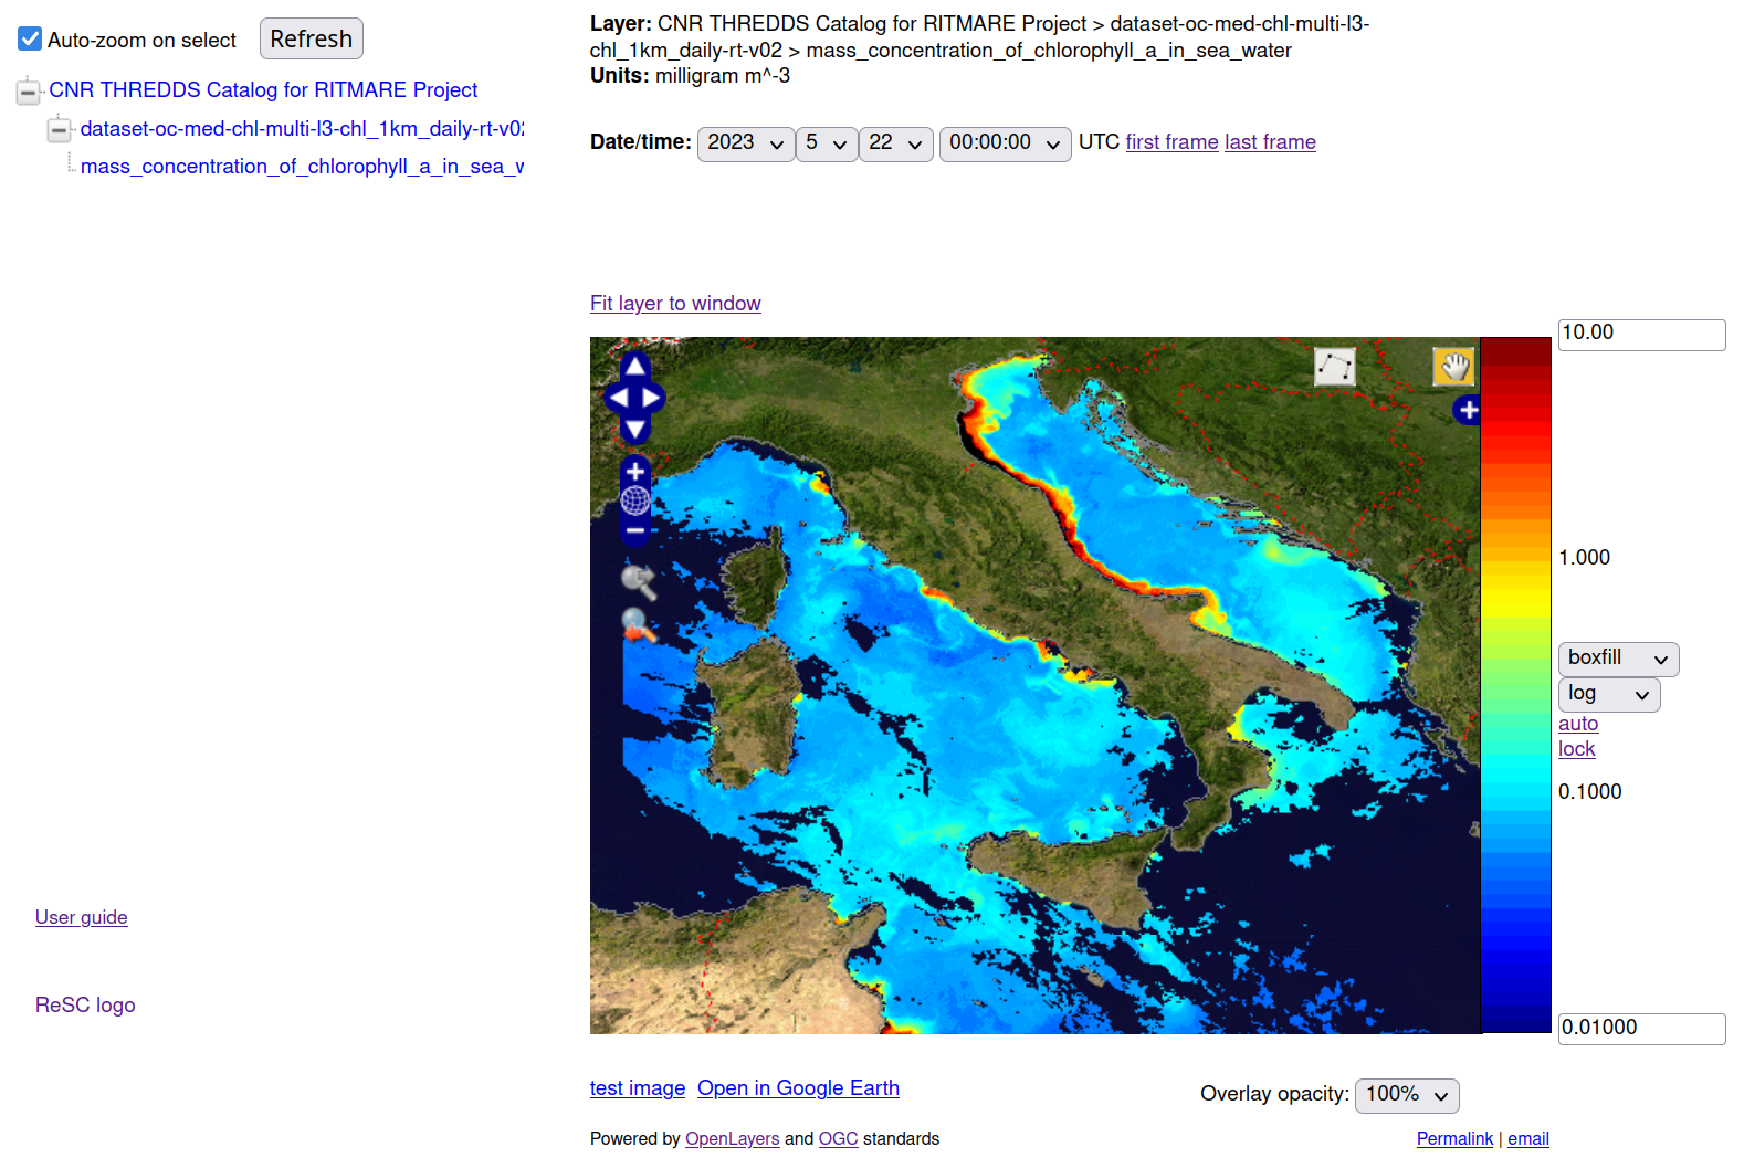
\includegraphics[width=\textwidth]{images/godiva_chla.pdf}
\captionsetup{font=small, hypcap=false}
\captionof{figure}{Chla rilevata in data 22 maggio 2023, visualizzazione tramite GODIVA2\footcite[Fonte: ][\url{http://ritmare.artov.ismar.cnr.it/thredds/godiva2/godiva2.html?menu=&layer=CHL&elevation=0&time=2023-05-22T00:00:00.000Z&scale=0.01,10&bbox=-238.354357,-338.673427,481.645643,223.826573&server=http://ritmare.artov.ismar.cnr.it/thredds/wms/xchlcase12}]{img-godiva-chla}.}
\label{fig:godiva_chla}
\end{minipage}
\vspace{0.25cm}
\end{figure}

L'unica variabile osservata risulta essere la Chla, dunque non ci sarà bisogno di alcuna selezione nella fase di importazione.

%****************************************************************%
% sea surface temperature                                        %
%****************************************************************%
\paragraph{Sea surface temperature (SST).} 
Gli oceani svolgono un ruolo importante nel sistema climatico, in parte grazie alla loro capacità di accumulare calore. L'inerzia termica degli oceani viene comunicata all'atmosfera tramite energia scambiata sulla superficie del mare. Questi flussi energetici dipendono principalmente dalla \textit{temperatura della superficie del mare} (\textbf{SST}) unitamente alla temperatura dell'aria, umidità e nuvolosità. In ogni caso la SST, come variabile climatica, svolge un ruolo chiave nell'analisi della regolazione del clima e dei suoi fenomeni di variabilità\footcite[116]{DeserSST2010}. È utilizzata da alcuni sistemi di previsione ma anche, ed è questo il caso, da enti pubblici e privati che si occupano  dell'analisi dell'ambiente marino\footcite[334]{BUONGIORNONARDELLI2015334}. 

%\paragraph{Variabile osservata.} 
La SST è rilevata tramite l'elaborazione di immagini notturne acquisite sia sui satelliti geostazionari che in orbita polare\footcite[335]{BUONGIORNONARDELLI2015334}. Le osservazioni si concentrano nell'area geo-spaziale rappresentante il mare italiano, delimitata da:
\begin{itemize}
    \item \textit{Longitudine}: da 7.0 a 20.0 Risoluzione=0.012 gradi est
    \item \textit{Latitudine}: da 35.0 a 46.0 Risoluzione=0.012 gradi nord 
\end{itemize}

I dati sono misurati in $kelvin (\unit\kelvin)$, unità di temperatura termodinamica\footcite[87]{10.1039/9781847557889}. 

%\paragraph{Misurazioni.}
I dati sono disponibili in un catalogo THREDDS\footcite[\url{http://ritmare.artov.ismar.cnr.it/thredds/ritmare/SatelliteOS/SST/catalog.html?dataset=SSTUHR}]{thredds-sst}  aggiornato contenente le variabili osservate in formato standard NetCDF-4\footcite[19-47]{HFR_QC_JERICO}. È presente un visualizzatore web -- \textit{GODIVA2} -- che consente la visualizzazione grafica dei dati provenienti dal dataset\footcite{blower2009godiva2}. Un esempio è mostrato in \autoref{fig:godiva_sst}.

\begin{figure}[!ht]
\noindent\begin{minipage}{\textwidth}
\vspace{1cm}
\centering
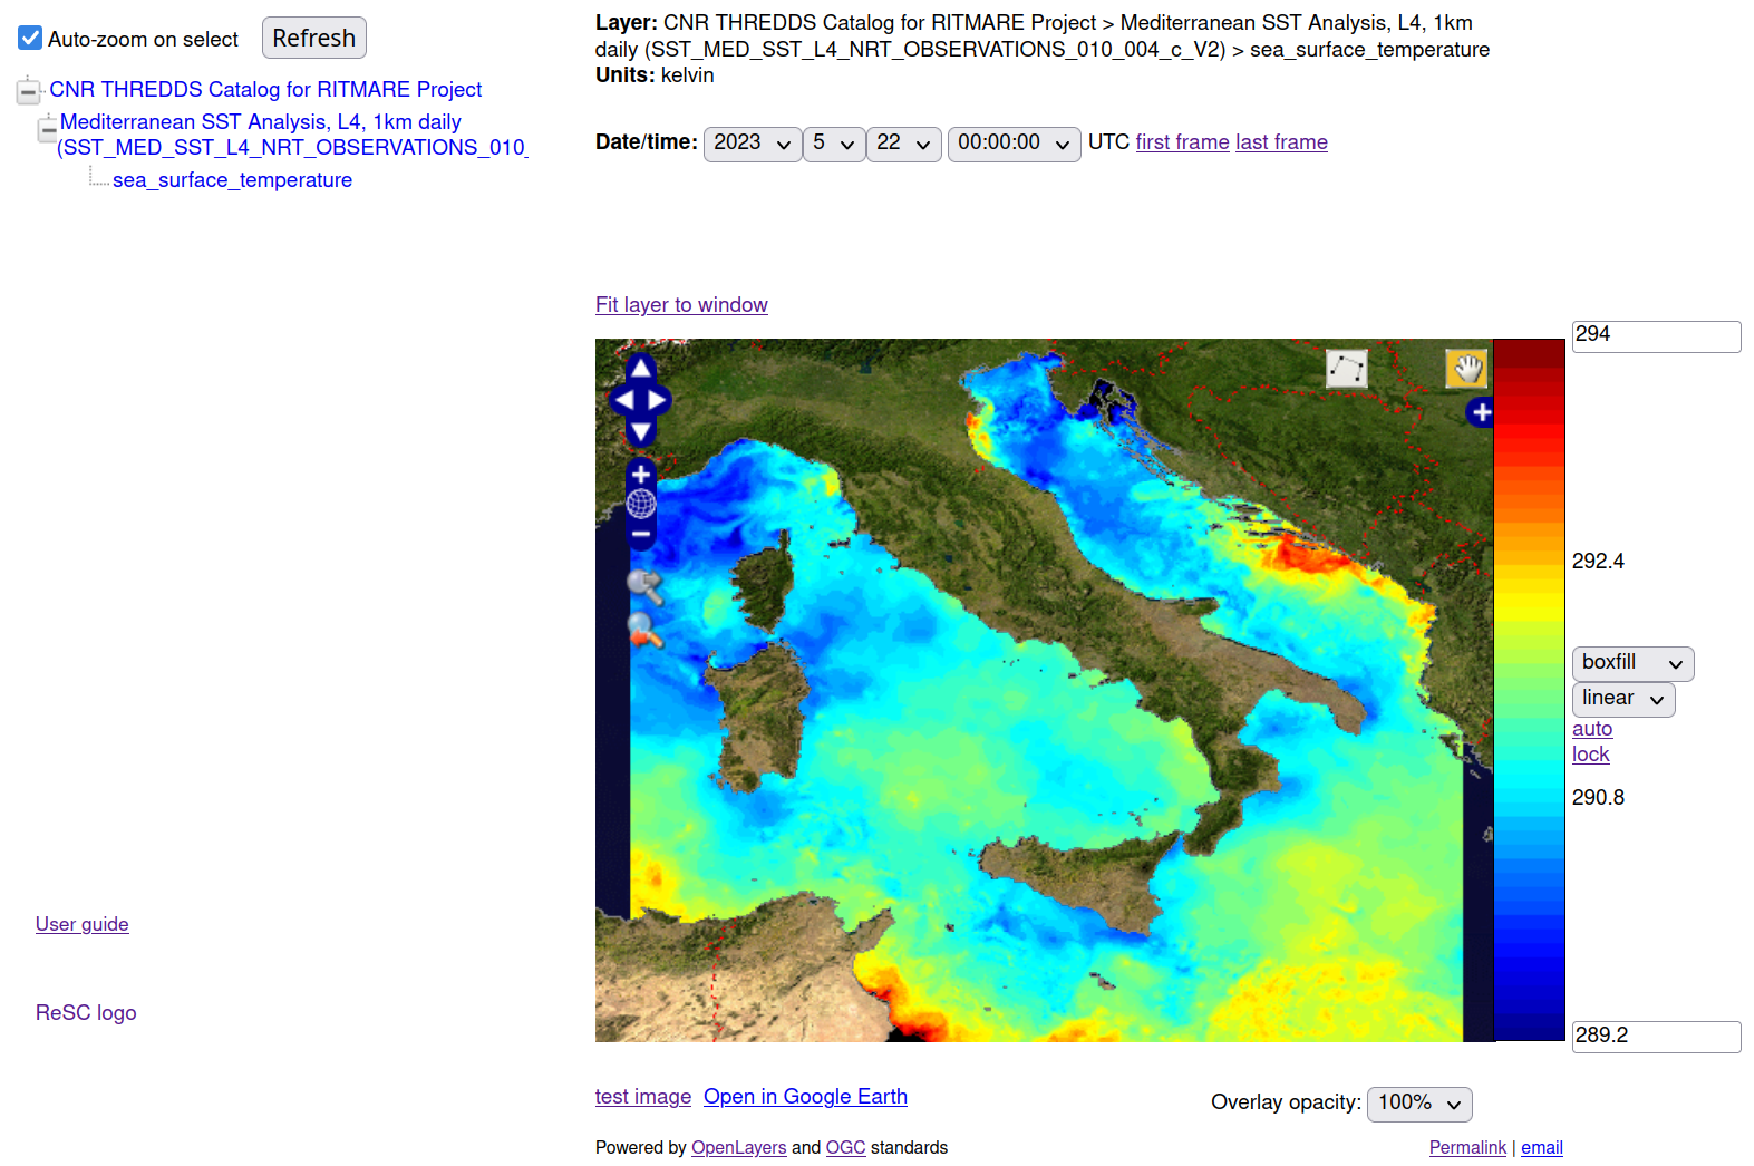
\includegraphics[width=\textwidth]{images/godiva_sst.pdf}
\captionsetup{font=small, hypcap=false}
\captionof{figure}{SST rilevata in data 22 maggio 2023, visualizzazione tramite GODIVA2\footcite[Fonte: ][\url{http://ritmare.artov.ismar.cnr.it/thredds/godiva2/godiva2.html?menu=&layer=analysed_sst&elevation=0&time=2023-05-22T00:00:00.000Z&scale=289.2,294&bbox=66.889391,84.287338,78.139391,93.0764&server=http://ritmare.artov.ismar.cnr.it/thredds/wms/sstuhr}]{img-godiva-sst}}
\label{fig:godiva_sst}
\end{minipage}
\vspace{0.25cm}
\end{figure}

L'unica variabile osservata risulta essere la SST, dunque non ci sarà bisogno di alcuna selezione nella fase di importazione.

\end{document}